\documentclass[10pt]{article}
\usepackage[polish]{babel}
\usepackage[utf8]{inputenc}
\usepackage[T1]{fontenc}
\usepackage{amsmath}
\usepackage{amsfonts}
\usepackage{amssymb}
\usepackage[version=4]{mhchem}
\usepackage{stmaryrd}
\usepackage{graphicx}
\usepackage[export]{adjustbox}
\graphicspath{ {./images/} }

\title{Instrukcja dla zdającego }

\author{}
\date{}


\begin{document}
\maketitle
\begin{center}
\begin{tabular}{|c|c}
\hline
MATEMATYKA - poziom rozszerzony &  \\
klasa II & CZERWIEC \\
\hline
\end{tabular}
\end{center}

Czas pracy:

\begin{enumerate}
  \item Sprawdź, czy arkusz egzaminacyjny zawiera 16 stron (zadania 1-17). Ewentualny brak zgłoś przewodniczącemu zespołu nadzorującego egzamin.
  \item Rozwiązania zadań i odpowiedzi wpisuj w miejscu na to przeznaczonym.
  \item Pamiętaj, że pominięcie argumentacji lub istotnych obliczeń w rozwiązaniu zadania otwartego może spowodować, że za to rozwiązanie nie otrzymasz pełnej liczby punktów.
  \item Pisz czytelnie i używaj tylko długopisu lub pióra z czarnym tuszem lub atramentem.
  \item Nie używaj korektora, a błędne zapisy wyraźnie przekreśl. Pamiętaj, że zapisy w brudnopisie nie będą oceniane.
  \item Możesz korzystać z zestawu wzorów matematycznych, cyrkla i linijki oraz kalkulatora prostego.
  \item Na karcie odpowiedzi wpisz swój numer PESEL
  \item Nie wpisuj żadnych znaków w części przeznaczonej dla egzaminatora.
\end{enumerate}

Liczba punktów do uzyskania:

W zadaniach o numerach od 1 do 5 wybierz i zaznacz na karcie odpowiedzi jedną poprawną odpowiedź

\section*{Zadanie 1. (1 pkt)}
Ile rozwiązań ma równanie: \(||x+3|-4|=2\) ?\\
A. 0\\
B. 2\\
C. 4\\
D. 6

\section*{Zadanie 2. (1 pkt)}
Reszta z dzielenia wielomianu \(W(x)=2 x^{3}+3 x^{2}-a x+1\) przez dwumian \(x+2\) jest równa -13.\\
A. \(a=-5\)\\
B. \(a=5\)\\
C. \(a=-2\)\\
D. \(a=2\)

\section*{Zadanie 3. (1 pkt)}
Jeżeli \(\sin \alpha=-\frac{1}{3} \quad \alpha \in\left(270^{\circ} ; 360^{\circ}\right)\) to:\\
A. \(\cos \left(90^{\circ}-\alpha\right)=\frac{-2 \sqrt{2}}{3}\)\\
B. \(\cos \left(90^{\circ}+\alpha\right)=\frac{2 \sqrt{2}}{3}\)\\
C. \(\operatorname{tg}\left(180^{\circ}-\alpha\right)=-\frac{\sqrt{2}}{4}\)\\
D. \(\operatorname{tg}\left(180^{\circ}+\alpha\right)=-\frac{\sqrt{2}}{4}\)

\section*{Zadanie 4. (1 pkt)}
Okrąg \((x+3)^{2}+(y-2)^{2}=25\) jest styczny do prostej:\\
A. \(x=-2\)\\
B. \(y=3\)\\
C. \(y=\frac{3}{4} x\)\\
D. \(y=\frac{3}{4} x-2\)

\section*{Zadanie 5. (1 pkt)}
Jeżeli \(\log _{2} 3=a\) wtedy \(\log _{2} 9+\log _{3} 16\) jest równe:\\
A. \(6 a\)\\
B. \(2 a+\frac{4}{a}\)\\
C. \(9 a+\frac{16}{a}\)\\
D. \(\frac{6}{a}\)

W zadaniach o numerach od 6 do 8 zakoduj we wskazanym miejscu wynik zgodnie z poleceniem.

\section*{Zadanie 6. (2pkt)}
W trójkącie kąt między bokami o długościach 8 i 6jest równy \(120^{\circ}\). Jaką długość ma trzeci bok trójkąta?\\
Zakoduj trzy pierwsze cyfry wyniku.\\

\includegraphics[max width=\textwidth, center]{2024_11_21_caad0d2d07cc5c30818fg-04}\\

\includegraphics[max width=\textwidth, center]{2024_11_21_caad0d2d07cc5c30818fg-04(1)}

Zadanie 7. (2pkt)\\
Określono ciąg wzorem rekurencyjnym: \(\left\{\begin{array}{l}a_{1}=6 \\ a_{n+1}=5 a_{n}-3\end{array}\right.\) Jaką wartość ma 5 wyraz tego ciągu? Wynik zakoduj.\\
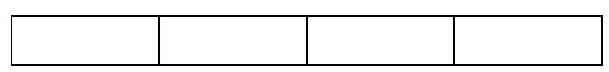
\includegraphics[max width=\textwidth, center]{2024_11_21_caad0d2d07cc5c30818fg-05}\\

\includegraphics[max width=\textwidth, center]{2024_11_21_caad0d2d07cc5c30818fg-05(1)}

Zadanie 8. (2pkt)\\
Przybliżenie z nadmiarem liczby x jest równe 15; błąd względny tego przybliżenia wynosi 0,025 . Wyznacz liczbę x.\\
Zakoduj cyfrę dziesiątek, jedności oraz pierwszą cyfrę rozwinięcia dziesiętnego.

\begin{center}
\begin{tabular}{|c|c|c|c|}
\hline
cyfra & dziesiątek & jedności & dziesiętne \\
\cline { 2 - 4 }
 &  &  &  \\
\hline
\end{tabular}
\end{center}

\begin{center}
\begin{tabular}{|c|c|c|c|c|c|c|c|c|c|c|c|c|c|c|c|c|c|c|c|c|c|c|c|c|c|c|c|c|c|c|}
\hline
 &  &  &  &  &  &  &  &  &  &  &  &  &  &  &  &  &  &  &  &  &  &  &  &  &  &  &  &  &  &  \\
\hline
 &  &  &  &  &  &  &  &  &  &  &  &  &  &  &  &  &  &  &  &  &  &  &  &  &  &  &  &  &  &  \\
\hline
 &  &  &  &  &  &  &  &  &  &  &  &  &  &  &  &  &  &  &  &  &  &  &  &  &  &  &  &  &  &  \\
\hline
 &  &  &  &  &  &  &  &  &  &  &  &  &  &  &  &  &  &  &  &  &  &  &  &  &  &  &  &  &  &  \\
\hline
 &  &  &  &  &  &  &  &  &  &  &  &  &  &  &  &  &  &  &  &  &  &  &  &  &  &  &  &  &  &  \\
\hline
 &  &  &  &  &  &  &  &  &  &  &  &  &  &  &  &  &  &  &  &  &  &  &  &  &  &  &  &  &  &  \\
\hline
 &  &  &  &  &  &  &  &  &  &  &  &  &  &  &  &  &  &  &  &  &  &  &  &  &  &  &  &  &  &  \\
\hline
 &  &  &  &  &  &  &  &  &  &  &  &  &  &  &  &  &  &  &  &  &  &  &  &  &  &  &  &  &  &  \\
\hline
 &  &  &  &  &  &  &  &  &  &  &  &  &  &  &  &  &  &  &  &  &  &  &  &  &  &  &  &  &  &  \\
\hline
 &  &  &  &  &  &  &  &  &  &  &  &  &  &  &  &  &  &  &  &  &  &  &  &  &  &  &  &  &  &  \\
\hline
 &  &  &  &  &  &  &  &  &  &  &  &  &  &  &  &  &  &  &  &  &  &  &  &  &  &  &  &  &  &  \\
\hline
 &  &  &  &  &  &  &  &  &  &  &  &  &  &  &  &  &  &  &  &  &  &  &  &  &  &  &  &  &  &  \\
\hline
 &  &  &  &  &  &  &  &  &  &  &  &  &  &  &  &  &  &  &  &  &  &  &  &  &  &  &  &  &  &  \\
\hline
 &  &  &  &  &  &  &  &  &  &  &  &  &  &  &  &  &  &  &  &  &  &  &  &  &  &  &  &  &  &  \\
\hline
 &  &  &  &  &  &  &  &  &  &  &  &  &  &  &  &  &  &  &  &  &  &  &  &  &  &  &  &  &  &  \\
\hline
 &  &  &  &  &  &  &  &  &  &  &  &  &  &  &  &  &  &  &  &  &  &  &  &  &  &  &  &  &  &  \\
\hline
 &  &  &  &  &  &  &  &  &  &  &  &  &  &  &  &  &  &  &  &  &  &  &  &  &  &  &  &  &  &  \\
\hline
 &  &  &  &  &  &  &  &  &  &  &  &  &  &  &  &  &  &  &  &  &  &  &  &  &  &  &  &  &  &  \\
\hline
 &  &  &  &  &  &  &  &  &  &  &  &  &  &  &  &  &  &  &  &  &  &  &  &  &  &  &  &  &  &  \\
\hline
 &  &  &  &  &  &  &  &  &  &  &  &  &  &  &  &  &  &  &  &  &  &  &  &  &  &  &  &  &  &  \\
\hline
 &  &  &  &  &  &  &  &  &  &  &  &  &  &  &  &  &  &  &  &  &  &  &  &  &  &  &  &  &  &  \\
\hline
 &  &  &  &  &  &  &  &  &  &  &  &  &  &  &  &  &  &  &  &  &  &  &  &  &  &  &  &  &  &  \\
\hline
 &  &  &  &  &  &  &  &  &  &  &  &  &  &  &  &  &  &  &  &  &  &  &  &  &  &  &  &  &  &  \\
\hline
 &  &  &  &  &  &  &  &  &  &  &  &  &  &  &  &  &  &  &  &  &  &  &  &  &  &  &  &  &  &  \\
\hline
 &  &  &  &  &  &  &  &  &  &  &  &  &  &  &  &  &  &  &  &  &  &  &  &  &  &  &  &  &  &  \\
\hline
 &  &  &  &  &  &  &  &  &  &  &  &  &  &  &  &  &  &  &  &  &  &  &  &  &  &  &  &  &  &  \\
\hline
 &  &  &  &  &  &  &  &  &  &  &  &  &  &  &  &  &  &  &  &  &  &  &  &  &  &  &  &  &  &  \\
\hline
 &  &  &  &  &  &  &  &  &  &  &  &  &  &  &  &  &  &  &  &  &  &  &  &  &  &  &  &  &  &  \\
\hline
 &  &  &  &  &  &  &  &  &  &  &  &  &  &  &  &  &  &  &  &  &  &  &  &  &  &  &  &  &  &  \\
\hline
 &  &  &  &  &  &  &  &  &  &  &  &  &  &  &  &  &  &  &  &  &  &  &  &  &  &  &  &  &  &  \\
\hline
 &  &  &  &  &  &  &  &  &  &  &  &  &  &  &  &  &  &  &  &  &  &  &  &  &  &  &  &  &  &  \\
\hline
 &  &  &  &  &  &  &  &  &  &  &  &  &  &  &  &  &  &  &  &  &  &  &  &  &  &  &  &  &  &  \\
\hline
 &  &  &  &  &  &  &  &  &  &  &  &  &  &  &  &  &  &  &  &  &  &  &  &  &  &  &  &  &  &  \\
\hline
 &  &  &  &  &  &  &  &  &  &  &  &  &  &  &  &  &  &  &  &  &  &  &  &  &  &  &  &  &  &  \\
\hline
 &  &  &  &  &  &  &  &  &  &  &  &  &  &  &  &  &  &  &  &  &  &  &  &  &  &  &  &  &  &  \\
\hline
 &  &  &  &  &  &  &  &  &  &  &  &  &  &  &  &  &  &  &  &  &  &  &  &  &  &  &  &  &  &  \\
\hline
 &  &  &  &  &  &  &  &  &  &  &  &  &  &  &  &  &  &  &  &  &  &  &  &  &  &  &  &  &  &  \\
\hline
 &  &  &  &  &  &  &  &  &  &  &  &  &  &  &  &  &  &  &  &  &  &  &  &  &  &  &  &  &  &  \\
\hline
 &  &  &  &  &  &  &  &  &  &  &  &  &  &  &  &  &  &  &  &  &  &  &  &  &  &  &  &  &  &  \\
\hline
 &  &  &  &  &  &  &  &  &  &  &  &  &  &  &  &  &  &  &  &  &  &  &  &  &  &  &  &  &  &  \\
\hline
 &  &  &  &  &  &  &  &  &  &  &  &  &  &  &  &  &  &  &  &  &  &  &  &  &  &  &  &  &  &  \\
\hline
\end{tabular}
\end{center}

Rozwiązania zadań od 9 do 18. należy zapisać w wyznaczonych miejscach pod treścią zadania.\\
Zadanie 9. (2 pkt)\\
Wykaż, że suma sześcianów trzech kolejnych liczb parzystych jest podzielna przez 24.

Zadanie 10. (3 pkt)\\
Wykaż, że w dowolnym trapezie do prostej łączącej środki podstaw należy punkt przecięcia przekątnych tego trapezu..\\

\includegraphics[max width=\textwidth, center]{2024_11_21_caad0d2d07cc5c30818fg-08}

Zadanie 11. (5 pkt)\\
Dla jakiej wartości parametru \(m \in R \quad f(x)=x^{2}+(m+1) x+3-m\) suma odwrotności kwadratów dwóch różnych miejsc zerowych funkcji \(f(x)\) jest większa od 1\\

\includegraphics[max width=\textwidth, center]{2024_11_21_caad0d2d07cc5c30818fg-09}

Odpowiedź:

Zadanie 12. (5 pkt)\\
Rozwiąż układ równań:\\
\(\left\{\begin{array}{l}2 x+3 y=4 \\ 4 x+m y=2 m\end{array}\right.\).\\
Dla jakich wartości parametru \(m\) rozwiązanie układu równań spełnia warunek: \(x \geq 0 \wedge y \geq 0\) ?\\

\includegraphics[max width=\textwidth, center]{2024_11_21_caad0d2d07cc5c30818fg-10}

Odpowiedź:

Zadanie 13. (4 pkt)\\
Z drutu o długości 200cm zbudowano ramkę w kształcie prostokąta. Jakie powinna mieć wymiary aby pole prostokąta było największe?\\

\includegraphics[max width=\textwidth, center]{2024_11_21_caad0d2d07cc5c30818fg-11}

Odpowiedź:

Zadanie 14. (4 pkt)\\
Na rysunku przedstawiono wykres funkcji \(f(x)\).\\
Naszkicuj wykres funkcji: \(g(x)=f(\mid x)-2\).\\
Określ dziedzinę oraz miejsca zerowe funkcji \(g(x) g(x)\)\\
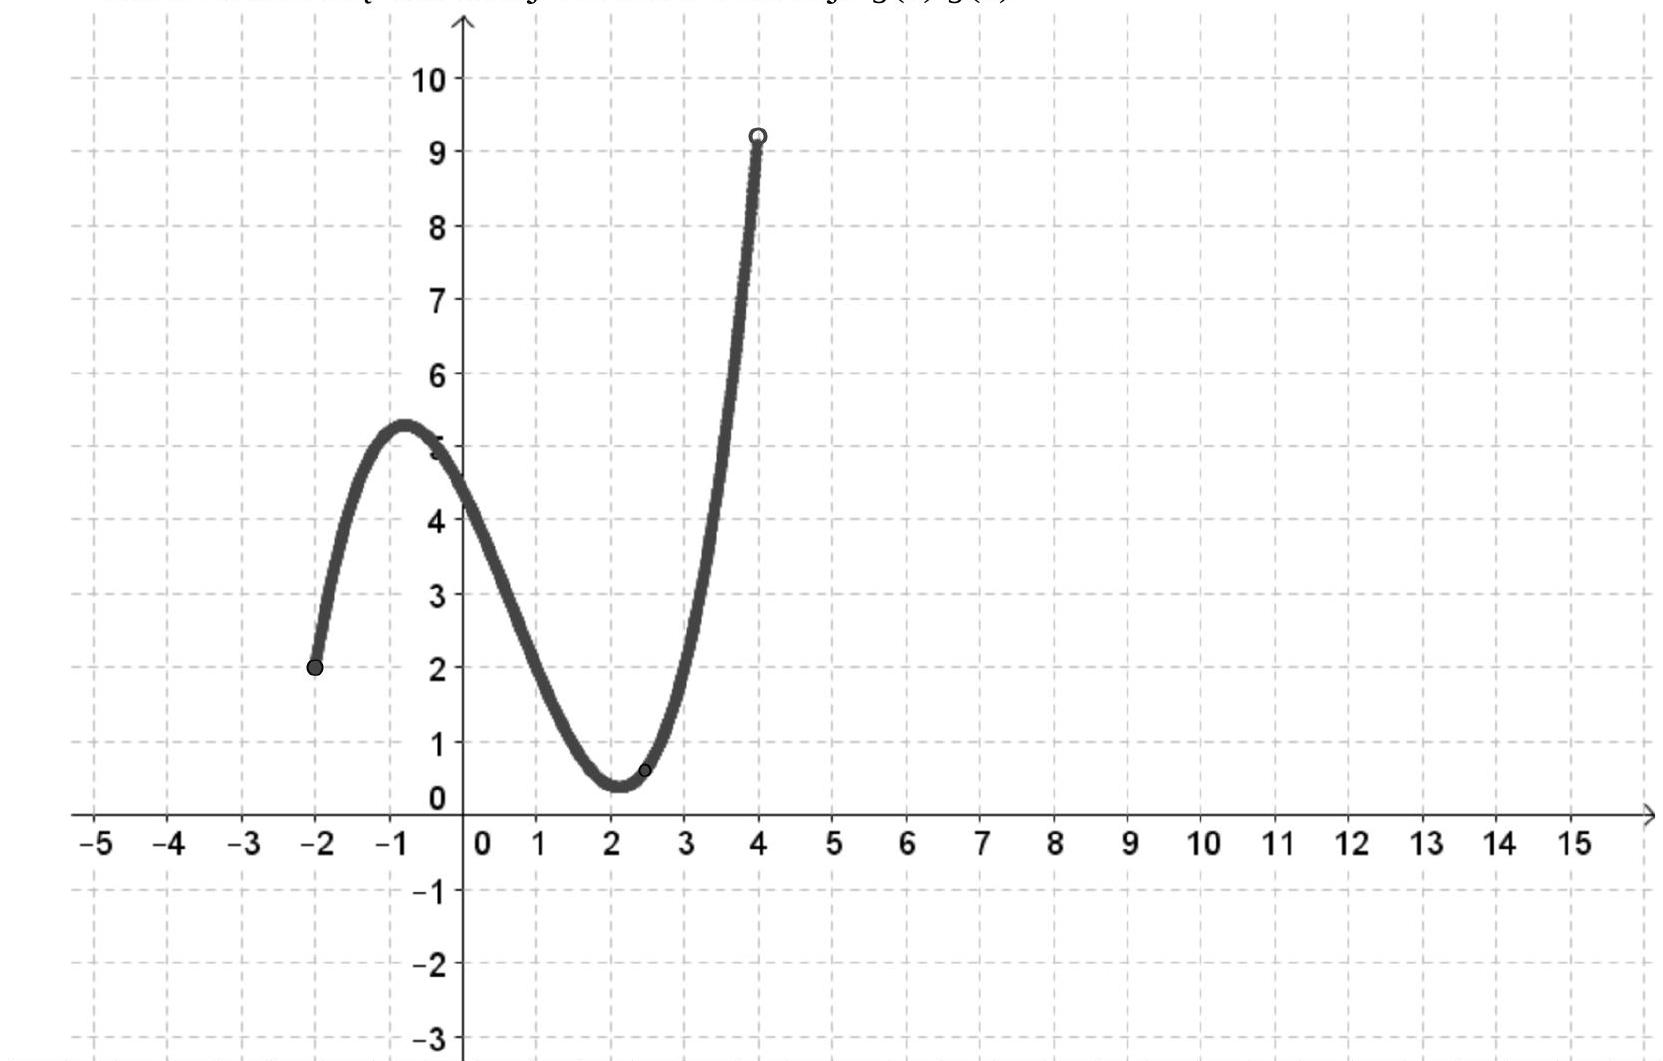
\includegraphics[max width=\textwidth, center]{2024_11_21_caad0d2d07cc5c30818fg-12}

\begin{center}
\begin{tabular}{|l|l|l|l|l|l|l|l|l|}
\hline
 &  &  &  &  &  &  &  &  \\
\hline
 &  &  &  &  &  &  &  &  \\
\hline
 &  &  &  &  &  &  &  &  \\
\hline
 &  &  &  &  &  &  &  &  \\
\hline
 &  &  &  &  &  &  &  &  \\
\hline
 &  &  &  &  &  &  &  &  \\
\hline
 &  &  &  &  &  &  &  &  \\
\hline
 &  &  &  &  &  &  &  &  \\
\hline
\end{tabular}
\end{center}

Odpowiedź:

Zadanie 15. (3 pkt)\\
Sprawdź czy równość jest tożsamością. Podaj odpowiednie założenia.\\
\(\frac{\sin \alpha}{1+\cos \alpha}+\frac{\sin \alpha}{1-\cos \alpha}=\frac{2}{\sin \alpha}\)\\

\includegraphics[max width=\textwidth, center]{2024_11_21_caad0d2d07cc5c30818fg-13}

Odpowiedź:

Zadanie 16. (4 pkt)\\
Wyznacz resztę z dzielenia wielomianu \(\mathrm{W}(\mathrm{x})\) przez wielomian \((x-1)(x+2)\) wiedząc, że \(W(1)=-1 \quad i \quad W(-2)=2\).\\

\includegraphics[max width=\textwidth, center]{2024_11_21_caad0d2d07cc5c30818fg-14}

Odpowiedź:

Zadanie 17. (5 pkt)\\
Trapez ABC jest wpisany w okrąg, przekątna AC jest zawarta w dwusiecznej kąta BAD, a długość podstawy AB jest dwa razy większa niż długość podstawy CD . Oblicz pole trapezu i obwód wiedząc że jego wysokość jest równa \(\sqrt{3}\).\\

\includegraphics[max width=\textwidth, center]{2024_11_21_caad0d2d07cc5c30818fg-15}

Odpowiedź:

Zadanie 18. (4 pkt)\\
Trzy liczby tworzą ciąg arytmetyczny o \(r=3\). Jeżeli pierwszą powiększymy o 8 drugą o 6 a trzecią pozostawimy bez zmian to otrzymamy trzy kolejne wyrazy ciągu geometrycznego. Znajdź te liczby.\\

\includegraphics[max width=\textwidth, center]{2024_11_21_caad0d2d07cc5c30818fg-16}

Odpowiedź:

WYPEENIA PISZĄCY

\begin{center}
\begin{tabular}{|l|c|c|c|c|}
\hline
\begin{tabular}{c}
Nr \\
zadania \\
\end{tabular} & A & B & C & D \\
\hline
1. & \(\square\) & \(\square\) & \(\square\) & \(\square\) \\
\hline
2. & \(\square\) & \(\square\) & \(\square\) & \(\square\) \\
\hline
3. & \(\square\) & \(\square\) & \(\square\) & \(\square\) \\
\hline
4. & \(\square\) & \(\square\) & \(\square\) & \(\square\) \\
\hline
\(\mathbf{5 .}\) & \(\square\) & \(\square\) & \(\square\) & \(\square\) \\
\hline
\end{tabular}
\end{center}

\section*{Suma punktów}
zadania zamknięte

WYPEENIA SPRAWDZAJACY

\begin{center}
\begin{tabular}{|l|c|c|c|}
\hline
\begin{tabular}{c}
\(\mathbf{N r}\) \\
zadania \\
\end{tabular} & \(\mathbf{X}\) & \(\mathbf{0}\) & \(\mathbf{2}\) \\
\hline
\(\mathbf{6 .}\) & \(\square\) & \(\square\) & \(\square\) \\
\hline
7. & \(\square\) & \(\square\) & \(\square\) \\
\hline
\(\mathbf{8 .}\) & \(\square\) & \(\square\) & \(\square\) \\
\hline
\end{tabular}
\end{center}

\begin{center}
\begin{tabular}{|l|c|c|c|c|c|c|c|c|}
\hline
\begin{tabular}{c}
\(\mathbf{N r}\) \\
zadania \\
\end{tabular} & \(\mathbf{X}\) & \(\mathbf{0}\) & \(\mathbf{1}\) & \(\mathbf{2}\) & \(\mathbf{3}\) & \(\mathbf{4}\) & \(\mathbf{5}\) & \(\mathbf{6}\) \\
\hline
\(\mathbf{9 .}\) & \(\square\) & \(\square\) & \(\square\) & \(\square\) &  &  &  &  \\
\hline
\(\mathbf{1 0 .}\) & \(\square\) & \(\square\) & \(\square\) & \(\square\) & \(\square\) &  &  &  \\
\hline
\(\mathbf{1 1 .}\) & \(\square\) & \(\square\) & \(\square\) & \(\square\) & \(\square\) & \(\square\) & \(\square\) &  \\
\hline
\(\mathbf{1 2 .}\) & \(\square\) & \(\square\) & \(\square\) & \(\square\) & \(\square\) & \(\square\) & \(\square\) &  \\
\hline
\(\mathbf{1 3 .}\) & \(\square\) & \(\square\) & \(\square\) & \(\square\) & \(\square\) & \(\square\) &  &  \\
\hline
\(\mathbf{1 4 .}\) & \(\square\) & \(\square\) & \(\square\) & \(\square\) & \(\square\) & \(\square\) &  &  \\
\hline
\(\mathbf{1 5 .}\) & \(\square\) & \(\square\) & \(\square\) & \(\square\) & \(\square\) &  &  &  \\
\hline
\(\mathbf{1 6 .}\) & \(\square\) & \(\square\) & \(\square\) & \(\square\) & \(\square\) & \(\square\) & \(\square\) &  \\
\hline
\(\mathbf{1 7 .}\) & \(\square\) & \(\square\) & \(\square\) & \(\square\) & \(\square\) & \(\square\) &  &  \\
\hline
\(\mathbf{1 8 .}\) & \(\square\) & \(\square\) & \(\square\) & \(\square\) & \(\square\) & \(\square\) &  &  \\
\hline
\end{tabular}
\end{center}

\begin{center}
\begin{tabular}{|c|}
\hline
\begin{tabular}{c}
Suma punktów \\
zadania otwarte \\
\end{tabular} \\
\hline
 \\
\hline
\end{tabular}
\end{center}

\begin{center}
\begin{tabular}{|c|c|}
\hline
\begin{tabular}{c}
Suma punktów \\
razem \\
\end{tabular} &  \\
\hline
 &  \\
\hline
\end{tabular}
\end{center}


\end{document}